\section{Menger-Problem}

\texttt{MENGER PROBLEM}:
\begin{itemize}
	\item \textbf{Gegeben}: Graph $G = (V, E)$ und $s, t\in V$
	\item \textbf{Gesucht}: Maximale Anzahl \textbf{kantendisjunkter} $s$-$t$-Pfade in $G$
\end{itemize}

Kann im Allgemeinen mit \texttt{MAX FLOW} gelöst werden, indem jede Kante Kapazität 1 erhält. Wenn Fluss $k$ ist, dann gibt es $k$ kantendisjunkte Wege. Laufzeit für planare Graphen liegt dann in $\mathcal{O}(n\log n)$.

Wir werden aber eine Lösung in Linearzeit kennenlernen.\\
\pagebreak

\textbf{Algorithmus für das \texttt{MENGER PROBLEM}}:

Sei o.B.d.A. $t$ an der äußeren Facette von $G$.
\begin{enumerate}
	\item Konstruiere gerichteten Graphen $D_1=(V,A_1)$ mit $uv\in A_1\iff uv\in E$
	\item Konstruiere $D_2=(V,A_2)$ aus $D_1$, sodass $D_2$ keine gerichteten Kreise im Uhrzeigersinn (Rechtskreise) enthält
	\item Finde maximale Anzahl gerichteter, kantendisjunkter $s$-$t$-Pfade $P_1,\ldots,P_k$ in $D_2$
	\begin{center}
		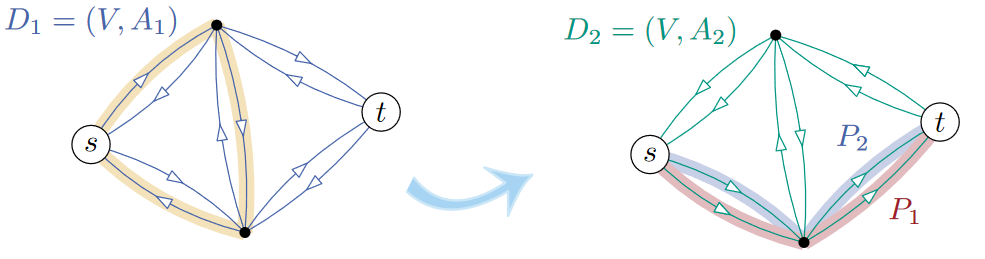
\includegraphics[width=0.5\textwidth]{images/menger-2.png}
	\end{center}
	\item Berechne aus $P_1,\ldots,P_k$ ungerichtete $s$-$t$-Pfade $Q_1,\ldots,Q_k$ in $G$
\end{enumerate}
\bigskip
Zeige \textbf{Korrektheit von Schritt 1}. Laufzeit und Durchführung sind klar.

\textbf{Lemma}: $G$ hat $k$ kantendisjunkte $s$-$t$-Pfade $\iff$ $D_1$ hat $k$ kantendisjunkte gerichtete $s$-$t$-Pfade

\textit{Beweis}: 
\begin{itemize}
	\item Gegeben $k$ kantendisjunkte gerichtete $s$-$t$-Pfade in D1, interpretiere diesen als Fluss $\Phi$ von Wert $k$ auf $D_1$ mit $\Phi(uv)\in\{0,1\}$ für jede gerichtete Kante
	\item Definiere $\Phi'$ als
	\begin{itemize}
		\item $\Phi'(uv)=\Phi'(vu)=0$, wenn $\Phi(uv)=\Phi(vu)=1$
		\item Ansonsten $\Phi'(uv)=\Phi(uv)$
		\item Es wurde der Fluss also dort auf 0 gesetzt, wo hin und Rückkante benutzt werden
	\end{itemize}
	\item $\Phi'$ hat Wert $k$ und es gibt $k$ kantendisjunkte Wege in $G$
	\begin{center}
		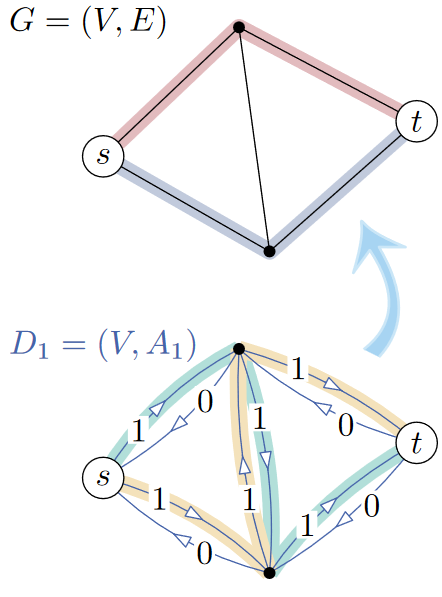
\includegraphics[width=0.2\textwidth]{images/menger-1.png}
	\end{center}
\end{itemize}
\bigskip
Nun wird die \textbf{Konstruktion in Schritt 2} beschrieben:
\begin{itemize}
	\item Betrachte Breitensuche von der äußeren Facette $f_0$ im gerichteten Dualgraphen $D_1^*$ von $D_1$
	\item Auf Level $i$ sind alle Facetten mit Abstand $i$ zu $f_0$. Drehe für jedes $i$ die Richtung aller gerichteten Kanten von Level $i$ nach Level $i+1$ um.
	\item Ergebnis: $D_2^*$ mit primalen Graph $D_2$
	\item Da Breitensuche in Linearzeit möglich ist, ist auch dieses Verfahren in Linearzeit möglich.
	\begin{center}
		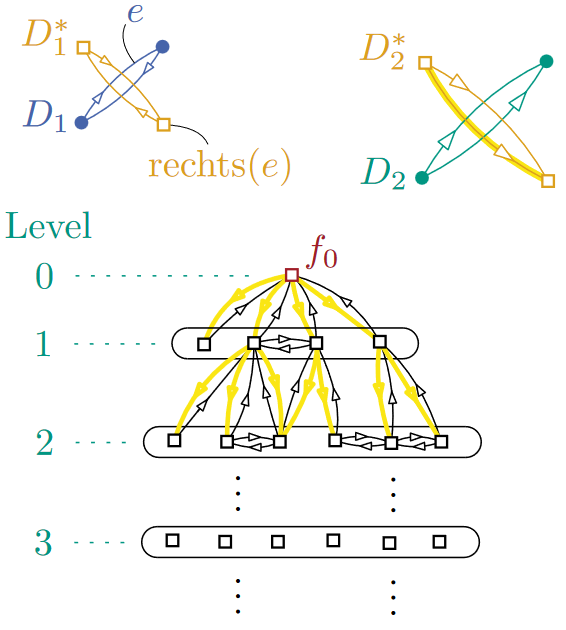
\includegraphics[width=0.3\textwidth]{images/menger-3.png}
	\end{center}
\end{itemize}

\textbf{Lemma}: $D_2$ enthält keine Rechtskreise

\textit{Beweis}: 
\begin{itemize}
	\item Angenommen $K$ wäre ein Rechtskreis in $D_2$
	\item Dann ist $K^*$ ein gerichteter Schnitt in $D_2^*$
	\item Sei $f$ eine Facette innerhalb von $K$
	\item Ein kürzester Weg von $f_0$ zu $f$ muss den Schnitt passieren, aber diese Kanten wurden in $D_2^*$ umgedreht.
	\item Widerspruch dazu, dass $K$ ein Rechtskreis ist
	\begin{center}
		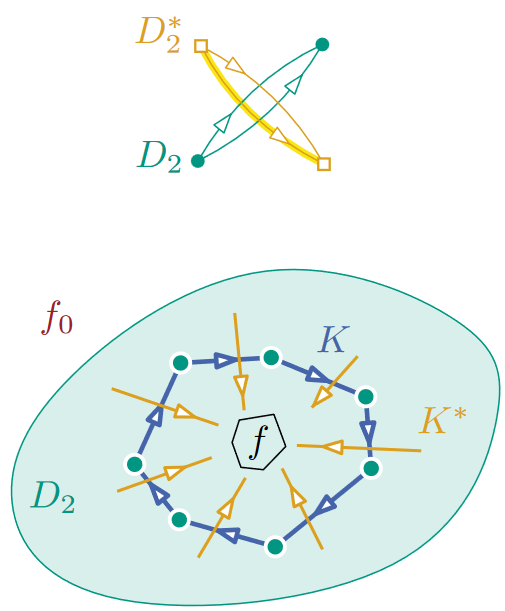
\includegraphics[width=0.25\textwidth]{images/menger-4.png}
	\end{center}
\end{itemize}

\textbf{Lemma}: $D_2$ enthält $k$ kantendisjunkte $s$-$t$-Wege $\iff$ $D_1$ enthält $k$ kantendisjunkte $s$-$t$-Wege.

\textit{Beweis}:
\begin{itemize}
	\item In Schritt 2 wurden im Dualen immer Kantenmengen zwischen zwei Levels umgedreht
	\item Das sind im Dualen $D_1^*$ knoteninduzierte $s$-$t$-Schnitte
	\item Im Primalen $D_1$ sind das für ein festes Level eine disjunkte Vereinigung von Kreisen
	\item Es reicht also zu zeigen, dass $k$ kantendisjunkte Wege, erhalten bleiben wenn ein gerichteter Kreis umgedreht wird
	\item Sei also ein gerichteter Kreis umgedreht
	\item Interpretiere wieder $k$ Wege als Fluss $\Phi$ mit Wert $k$
	\item Drehe Orientierung der Kanten und gleichzeitig den Flusswert der Kante
	\item Dies erhält die Flusseigenschaften und wir erhalten wieder ein Fluss $\Phi'$ mit Wert $k$ $\implies$ Wir erhalten auch wieder $k$ Wege.
	\begin{center}
		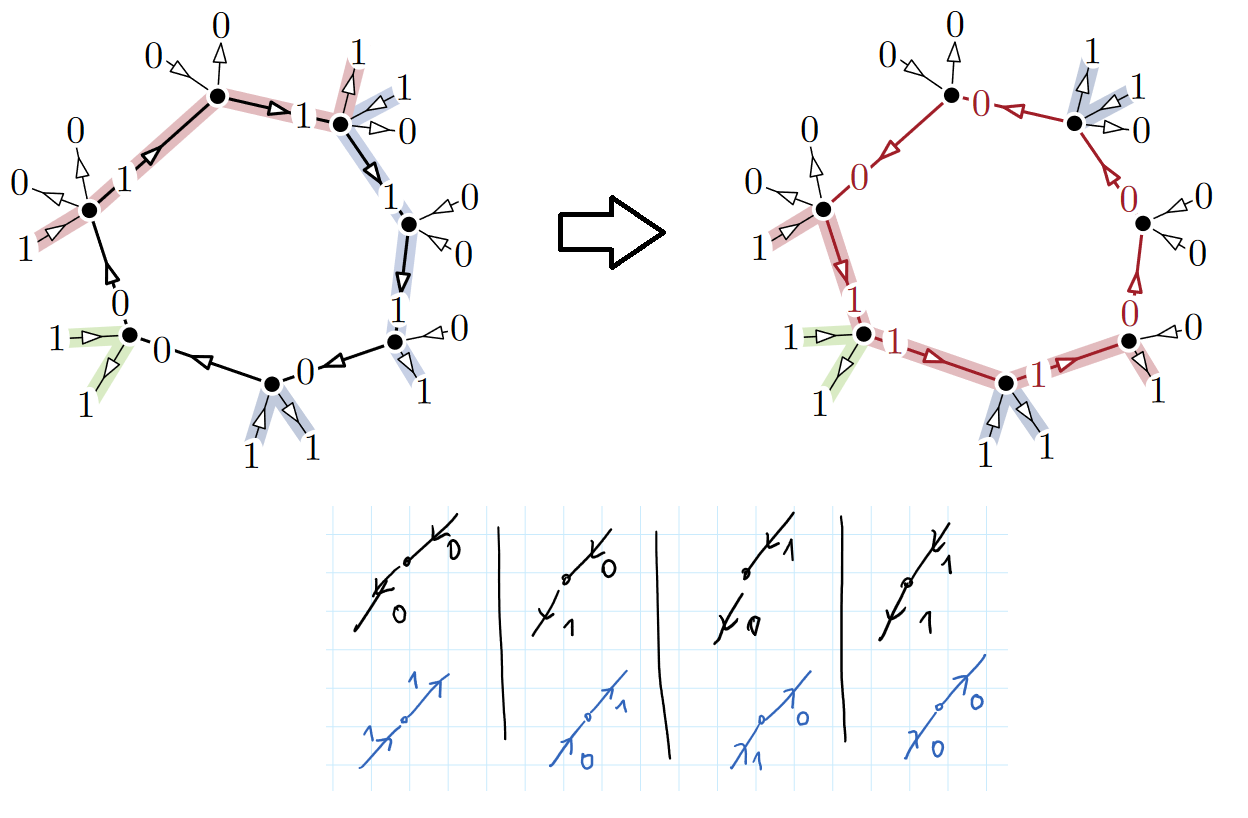
\includegraphics[width=0.5\textwidth]{images/menger-5.png}
	\end{center}
\end{itemize}
\bigskip
Nun wird das \textbf{Vorgehen in Schritt 3} beschrieben:
\begin{itemize}
	\item Jeder Knoten in $D_2$ hat gleich viele eingehende wie ausgehende Kanten, da das in $D_1$ der Fall war und in Schritt 2 nur Kreise umgedreht wurden, was die Eigenschaft weiterhin erhält
	\item Starte Tiefensuche bei $s$ mit ausgehender Kante
	\item Nimm immer die rechteste ausgehende Kante bzgl. der gerade genommenen eingehenden Kante und gehe über jede Kante nur einmal
	\item Wenn $t$ erreicht wird, ist ein $s$-$t$-Pfad gefunden und man fängt wieder bei $s$ mit neuer Kante an
	\item Aufhören wenn keine ausgehende Kante verfügbar ist (das passiert bei $s$)
	\item Wenn Knoten $t$ insgesamt $k$-mal erreicht wurde, wurden $k$ kantendisjunkte $s$-$t$-Pfade gefunden.
	\begin{center}
		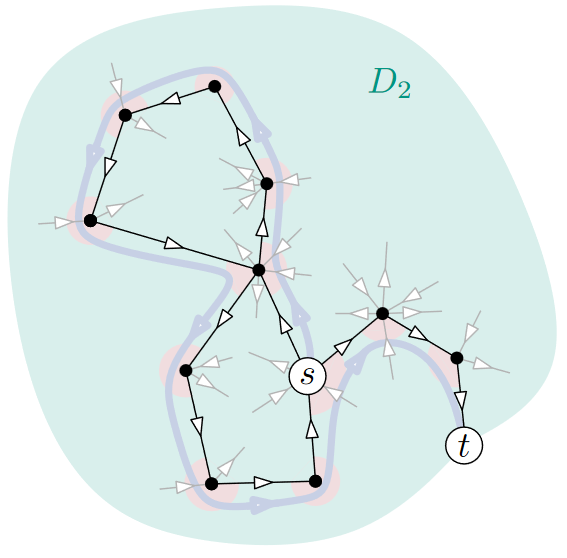
\includegraphics[width=0.3\textwidth]{images/menger-6.png}
	\end{center}
\end{itemize}

\textbf{Laufzeit von Schritt 3}:
\begin{itemize}
	\item Rechteste Kante kann mit Union-Find-Datenstruktur gefunden werden
	\item Laufzeit von Union-Find ist allgemein $\mathcal{O}(n\cdot\alpha(n))$, also nur fast linear
	\item Hier Spezialfall, in dem $n$ Operationen vom Typ Union und Find in Linearzeit ausgeführt werden können $\rightarrow$ Insgesamt Linearzeit
\end{itemize}

\textbf{Korrektheit von Schritt 3}:
\begin{itemize}
	\item \textbf{Ziel}: Finde einen $s$-$t$-Schnitt dessen Kapazität der Anzahl $k$ der gefundenen $s$-$t$-Pfade entspricht. Dann kann es nicht mehr als $k$ kantendisjunkte Pfade von $s$ nach $t$ geben, da diese den Schnitt passieren müssen
	\item Betrachte Graphen $D = (V, A)$ mit allen Kanten, die im Algorithmus genommen wurden
	\item Starte Tiefensuche in $D$ bei $s$ aber gehe Kanten rückwärts und nehme die linkeste mögliche Fortsetzung
	\item Baue damit rückwärts einen gerichteten Weg $W$ zu $s$ auf und stoppe, wenn wir eine Kante aus $W$ als Fortsetzung nehmen würden oder wenn wir wieder auf $s$ treffen
	\item Wir treffen nicht auf $t$, da $t$ in $D$ keine ausgehenden Kanten hat. Außerdem bleiben wir nicht hängen, da alle anderen Knoten so viele eingehende wie ausgehende Kanten haben
	\begin{center}
		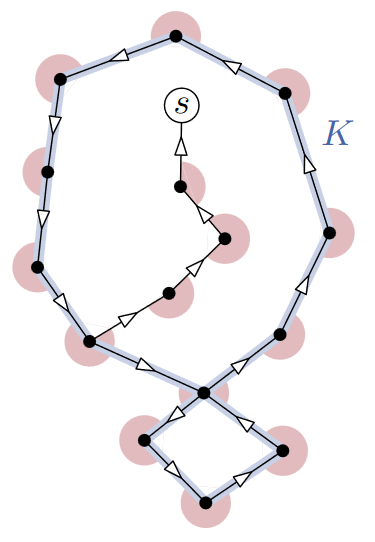
\includegraphics[width=0.2\textwidth]{images/menger-7.png}
	\end{center}
	\item $W$ umschließt ein Gebiet, dessen Rand $K$ eine Menge gerichteter Kreise ist
	\item Entlang von $K$ sind auf der rechten Seite Winkel ohne eingehenden Kanten
	\item Wegen Schritt 2 hat $K$ keinen Rechtskreis $\rightarrow$ Winkel sind außen an den Kreisen
	\item Also muss $s$ entweder auf $K$ oder $\text{int}(K)$ liegen, da (Rückwärts-)Wege von $s$ zu den Knoten in $K$ existieren und diese nicht in die Winkel laufen können
	\item Knoten $t$ liegt nicht auf $K$, da er ohne ausgehende Kante nicht von der Rückwärts-Tiefensuche gefunden werden kann. $t\in\text{ext}(K)$, da $t$ nach Annahme auf der äußeren Facette von $D$ liegt
	\item Definiere nun $S\subseteq V$ als Menge aller Knoten auf $K$ und in $\text{int}(K)$. $S$ induziert unseren $s$-$t$-Schnitt $C\subseteq A_2$
	\item \textbf{Zu zeigen}: Kapazität $c(C)\leq k$
	\item \textbf{Fall 1}: Sei $uv\in A$ mit $u\in V(K)$ und $v\in V-S$ eine Kante, die vom Algo benutzt wurde
	\begin{center}
		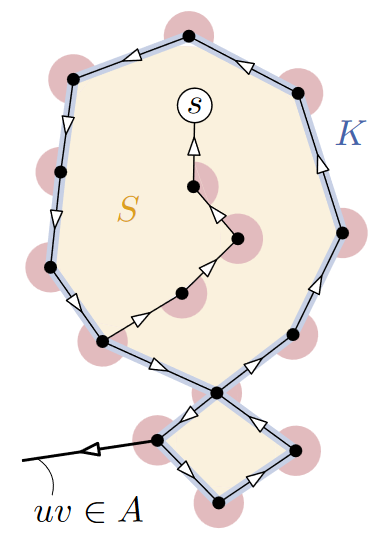
\includegraphics[width=0.2\textwidth]{images/menger-8.png}
	\end{center}
	\begin{itemize}
		\item Dann ist die Tiefensuche nach $uv$ nicht wieder nach $S$ gekommen, endete also in $t$, denn Winkel haben keine eingehenden Kanten aus $A$!
		\item Es gibt also höchstens $k$ solcher Kanten!
	\end{itemize}
	\item \textbf{Fall 2}: Sei $uv\in A_2-A$ Kante mit $u\in V(K)$ und $v\in V-S$, die vom Algo nicht benutzt wurde:
	\begin{center}
		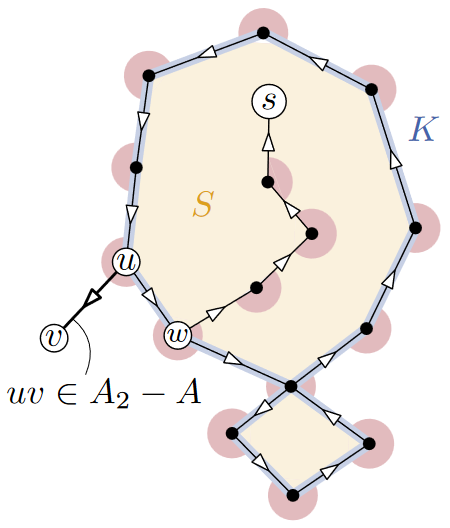
\includegraphics[width=0.22\textwidth]{images/menger-9.png}
	\end{center}
	\begin{itemize}
		\item Betrachte $uw\in E(K)$, die benutzt wurde und deren benutzte Vorgängerkante $xu$. Dann ist $x\in S$, da keine benutzten eingehenden Kanten in Winkeln liegen
		\item Dann ist aber $uv$ eine bessere (weiter rechts) Fortsetzung für
		$xu$ als $uw$ $\rightarrow$ Widerspruch!
		\item Also gibt es keine solche Kanten!
	\end{itemize}
	\item In beiden Fällen hat der Schnitt also Kapazität höchstens $k$ und die Optimalität des Algorithmus ist bewiesen.
\end{itemize}

Damit wurde bewiesen, dass das \texttt{MENGER PROBLEM} in Linearzeit gelöst werden kann. Für Schritt 4 muss lediglich das Vorgehen aus Schritt 1 und 2 invertiert werden.
